% ════════════════════════════════════════════
%  Figures
% ════════════════════════════════════════════

\begin{figure}[ht]
\centering
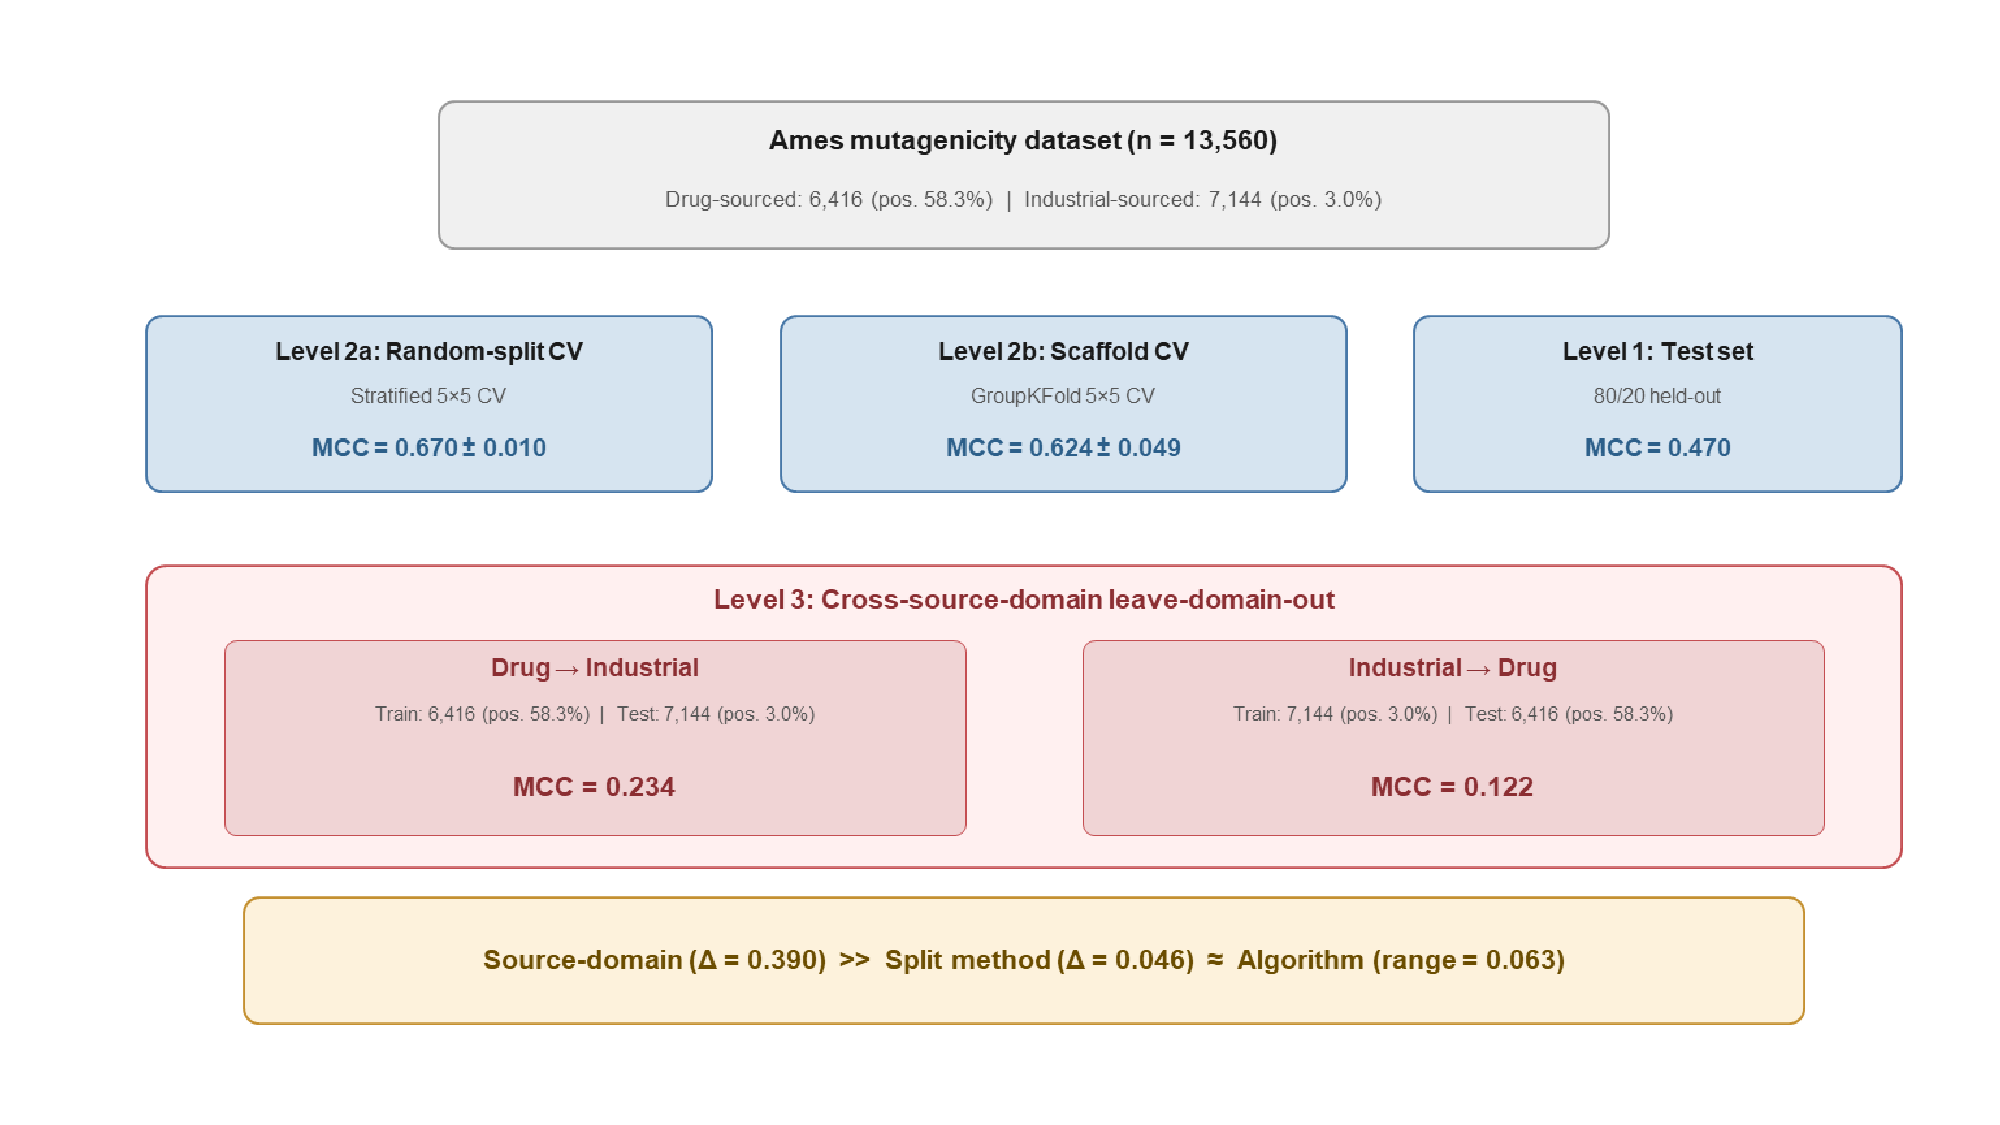
\includegraphics[width=\textwidth]{figures/figure1_framework.pdf}
\caption{Three-level evaluation framework for genotoxicity QSAR. All three levels use the same locked configuration (XGBoost, compact features, raw SMILES) to enable fair comparison of MCC across evaluation methods. The overestimation hierarchy summarizes the relative magnitudes observed in this benchmark.}
\label{fig:framework}
\end{figure}

\begin{figure}[ht]
\centering
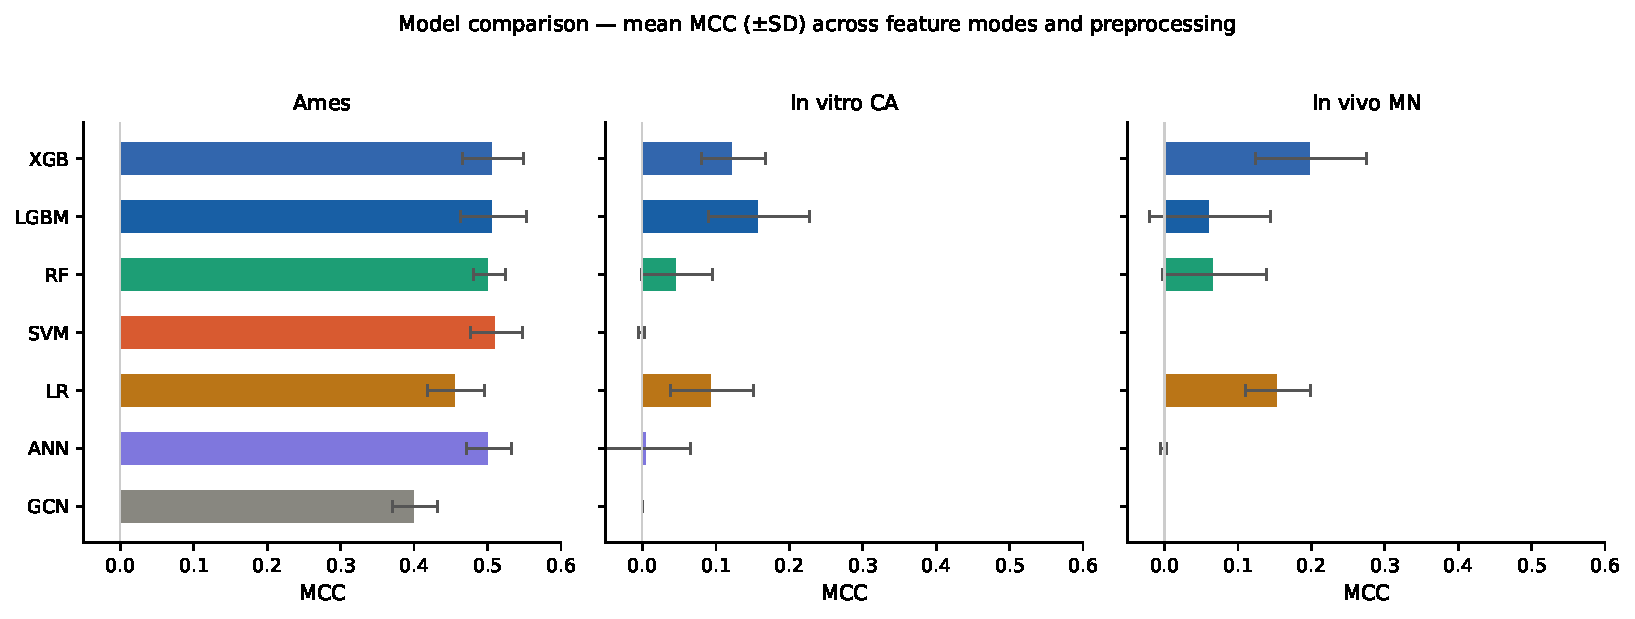
\includegraphics[width=\textwidth]{figures/figure2_model_comparison.pdf}
\caption{Mean MCC ($\pm$SD) by algorithm across all feature modes and preprocessing scenarios, grouped by endpoint. Error bars represent $\pm$1 SD. Within each endpoint, the top five tabular models show minimal performance spread (Ames range = 0.023 excluding LR and GCN).}
\label{fig:model_comparison}
\end{figure}

\begin{figure}[ht]
\centering
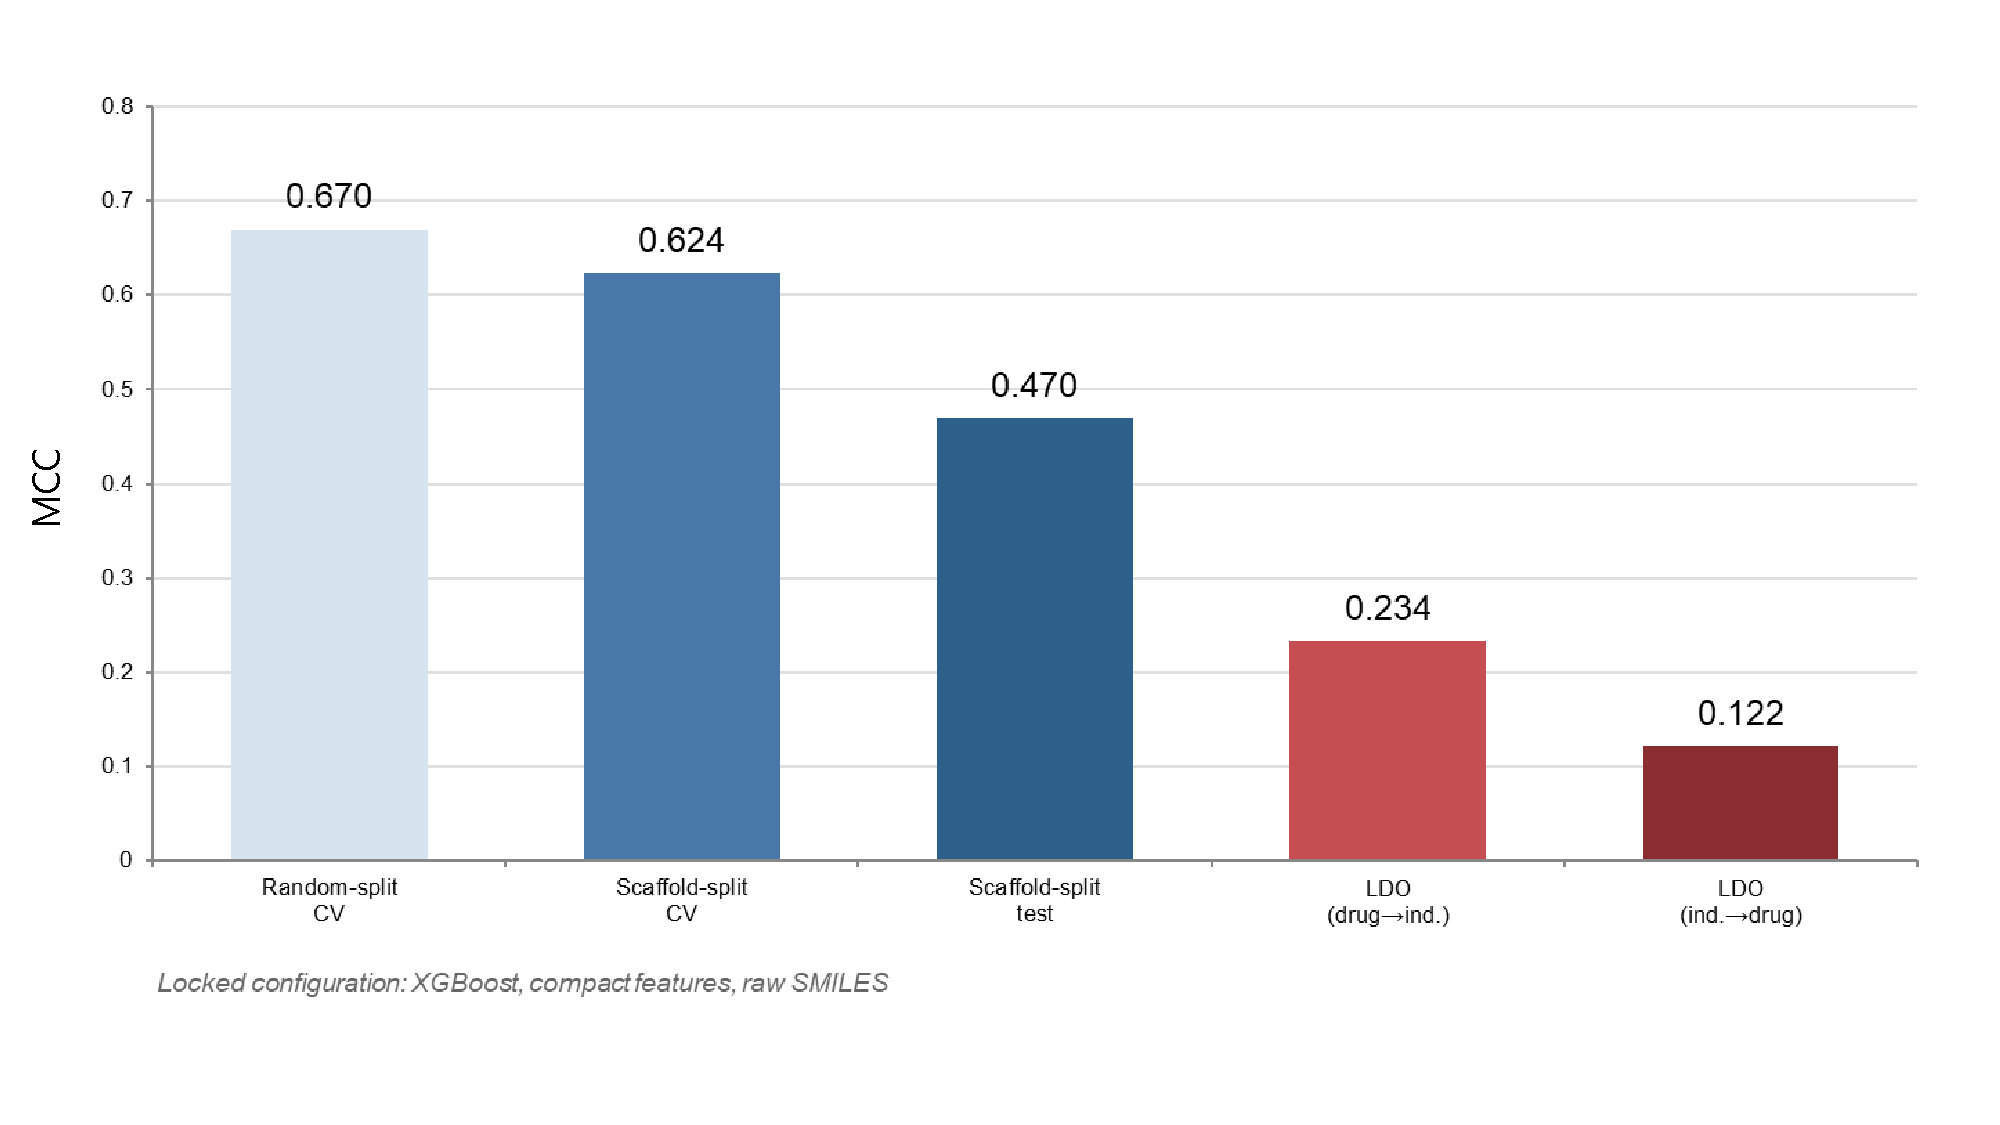
\includegraphics[width=0.85\textwidth]{figures/figure3_cascade.pdf}
\caption{Evaluation rigor cascade for Ames mutagenicity (locked configuration: XGBoost, compact features, raw SMILES). MCC decreases from random-split CV (0.670) through scaffold-split CV (0.624) and scaffold-split held-out test (0.470) to cross-source-domain LDO (0.234 drug$\to$industrial, 0.122 industrial$\to$drug). The source-domain effect ($\Delta = 0.390$, scaffold CV to LDO) substantially exceeds the split-method effect ($\Delta = 0.046$). All values from the same model, features, and preprocessing.}
\label{fig:cascade}
\end{figure}

\begin{figure}[ht]
\centering
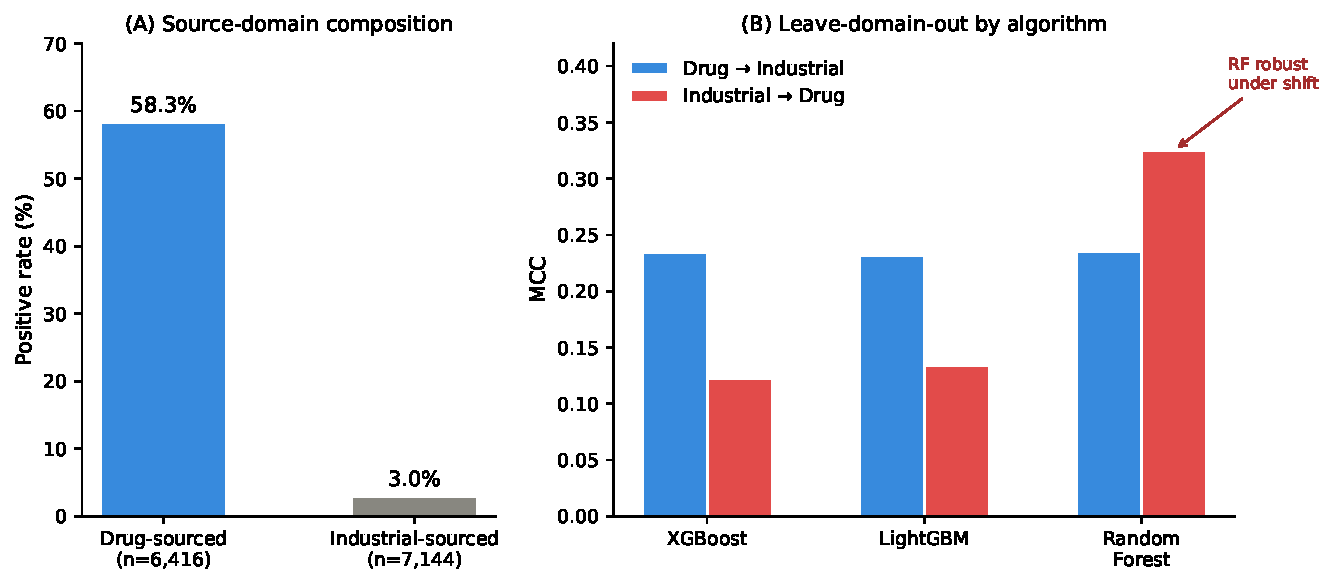
\includegraphics[width=\textwidth]{figures/figure4_domain_ldo.pdf}
\caption{Source-domain composition and cross-domain robustness in the Ames dataset. (A)~Positive rate by source domain: drug-sourced 58.3\% vs.\ industrial-sourced 3.0\% (19.5-fold difference). (B)~Leave-domain-out MCC for three algorithms. Drug$\to$industrial generalization is consistent across algorithms, but industrial$\to$drug direction reveals Random Forest's substantially better robustness (MCC = 0.325 vs.\ XGBoost 0.122).}
\label{fig:domain}
\end{figure}

\begin{figure}[ht]
\centering
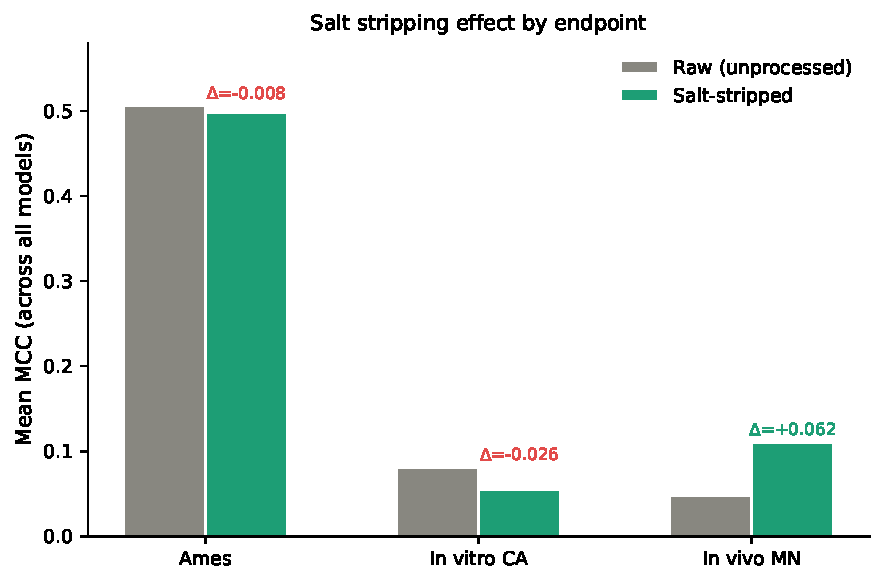
\includegraphics[width=0.75\textwidth]{figures/figure5_salt_stripping.pdf}
\caption{Effect of salt stripping on mean MCC (averaged across all models and feature modes) by endpoint. Salt stripping improved in~vivo mean MCC from 0.048 to 0.111 ($\Delta = +0.063$); the best individual in~vivo model showed a larger improvement of +0.225 (raw MCC = 0.086 $\to$ salt-stripped MCC = 0.311). Ames showed mixed effects; in~vitro showed a decrease.}
\label{fig:salt}
\end{figure}

\begin{figure}[ht]
\centering
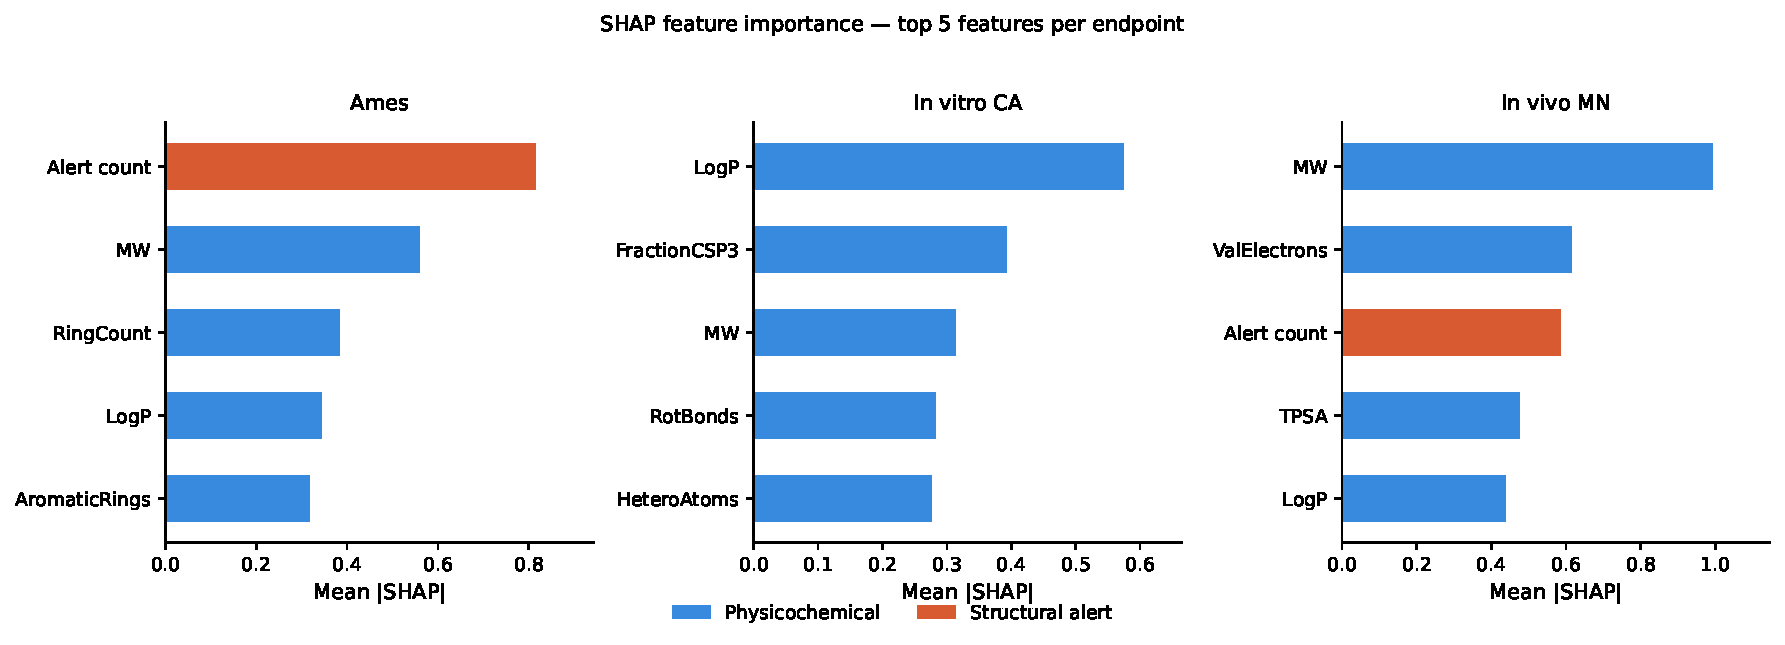
\includegraphics[width=\textwidth]{figures/figure6_shap.pdf}
\caption{SHAP feature importance (top 5 features) for each primary endpoint, computed from the best-performing tree-based model. Physicochemical descriptors (blue) dominate across all endpoints. Structural alert count (orange) ranks first for Ames but is absent from the in~vitro top 5. Individual fingerprint bits are absent from the top 5 for all endpoints despite comprising 50--75\% of features in the broad modes.}
\label{fig:shap}
\end{figure}

\begin{figure}[ht]
\centering
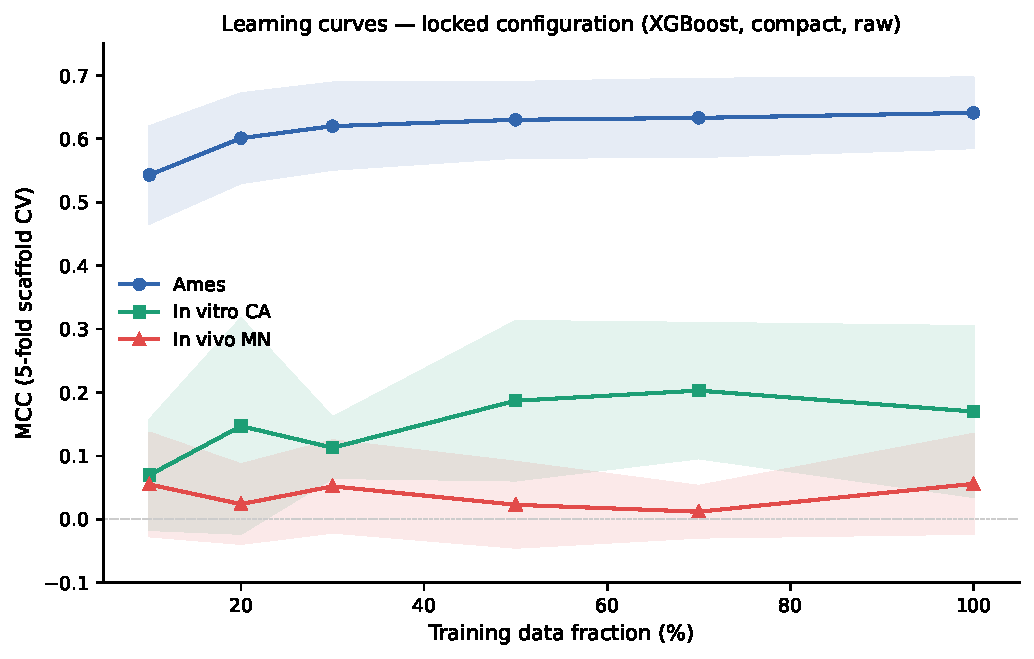
\includegraphics[width=0.8\textwidth]{figures/figure7_learning_curves.pdf}
\caption{Learning curves for the locked configuration (XGBoost, compact features, raw SMILES). Ames MCC saturates by 30\% of training data; in~vitro shows a noisy upward trend; in~vivo is flat throughout, indicating that additional data does not improve classification under this configuration. Shaded regions represent $\pm$1 SD across 5-fold scaffold CV. Note: the in~vivo curve reflects the locked configuration only; the best-performing salt-stripped configuration was not evaluated.}
\label{fig:learning_curves}
\end{figure}
